\documentclass{article}
\usepackage{parskip}
\usepackage{enumitem}
\usepackage{hyperref}
\usepackage[version=4]{mhchem}
\usepackage[margin=3cm]{geometry}
\usepackage{amsmath, amsthm, amssymb}
\usepackage{empheq}
\usepackage{pgfplots}
\usepackage{subcaption}
\usepackage{graphicx}
\usepackage{placeins}

\title{The Mathematics of Surface Enzyme Kinetics}
\author{William Tu}
\date{}

% new commands

\newcommand{\od}[2]{\frac{d #1}{d #2}}
\newcommand{\pd}[2]{\frac{\partial #1}{\partial #2}}
\newcommand{\GS}{\Gamma_\text{S}}
\newcommand{\GES}{\Gamma_{\text{ES}}}
\newcommand{\GP}{\Gamma_{\text{P}}}
\newcommand{\Et}{[\text{E}]_t}
\newcommand{\kcat}{k_{\text{cat}}}
\newcommand{\thetaP}{\theta_{\text{P}}}

% new theorems and lemmas
\newtheorem{lemma}{Lemma}

\pgfplotsset{compat=newest}
\usepgfplotslibrary{external}
\tikzexternalize

\begin{document}
\maketitle

\section{Introduction} \label{section:1}

In this report, we will be going over the chemical and mathematical framework we use to model our experimental results, explaining why the models are used, their advantages, and how one interprets them. Because we are using surface-attached substrates, the kinetic framework we use will be different from that used for substrates in solution. Ultimately, we will be able to obtain the product concentration as a function of time and hence fit the reaction progress curve to experimental data.

\section{Chemical framework} \label{section:2}

Throughout this report, we will use the Michaelis-Menten kinetics framework, which models enzymatic reactions in a relatively straightforward way. 

In words, the enzyme E reacts with the surface-attached substrate S and forms an enzyme-substrate complex ES. This is a reversible reaction, so both formation and dissociation are possible, with rate constants $k_1$ and $k_{-1}$, respectively. After the ES complex forms, it dissociates and yields the product P on the surface irreversibly, releasing enzyme E back into the solution. This is known as the catalysis reaction, with rate constant $\kcat$.

As a chemical equation \cite{wiki:michaelis}, we have

\begin{equation}
    \ce{E + S <=>[$k_1$][$k_{-1}$] ES ->[$\kcat$] P + E}
    \label{chem:reaction1}
\end{equation}

\section{Mathematical framework} \label{section:3}

For substrates in solution, the steady-state approximation is often used,  depending on two premises \cite{annedemaille12}:

\begin{enumerate}[label=(\roman*)]
    \item An ephemeral pre-steady state where only a small amount of ES complex forms.
    \item A steady state encompassing all of experimental time in which the concentration of the ES complex does not change, due to competing factors of complex formation, dissociation, consumption.
\end{enumerate}

The above premises hold for substrates in solution, which typically exceeds the enzyme concentration. However, the premises clearly do not hold for surface-attached substrates as they are in limited quantity, so the applicability of steady-state approximation is in this case questionable. Furthermore, there is a factor of diffusion due to the nature of the heterogeneous reaction which, if taken into account, produces very complex equations that are difficult to solve analytically. \cite{meena10}\cite{squires08} However, in practice, we can assume that the diffusional rate is negligible compared to that of the enzymatic reaction because in experiments, the diffusional rate can be made relatively fast, minimizing its contribution to the overall kinetics.

We can however, compare the theoretical predictions derived under the steady-state approximation framework and those without such approximation and determine whether the solution derived under steady-state approximation could match the exact solution, and if so, the mathematical conditions for which this is possible. This is exactly what we do below.

Before we head into the derivations, though, we setup the rate equations \cite{chemtalk24}\cite{wiki:steadystate} and initial conditions. From \eqref{chem:reaction1}, we have

\begin{empheq}[left=\empheqlbrace]{align}
    &\pd{\GS}{t} = k_{-1} \GES - k_1 \GS \Et  \label{maths:eq2} \\[5pt]
    &\pd{\GES}{t} = k_1 \GS \Et - (k_{-1} + \kcat) \GES 
    \label{maths:eq3} \\[5pt]
    &\pd{\GP}{t} = \kcat \GES \label{maths:eq4}
\end{empheq}

where the rate constants are defined above and $[\text{E}]_t$ is the bulk enzyme concentration, i.e. the "normal" concentration without diffusional effects. The initial conditions when $t = 0$: $\GS = \Gamma_0$, $\GES = \GP = 0$. 

Note that by the conservation of reaction "sites" on the electrode, 

\begin{equation}
    \GS + \GES + \GP = \Gamma_0
    \label{maths:eq5}
\end{equation}

\section{Derivation of the steady-state solution} \label{section:4}

Note that the goal is to derive an expression for $\GP$.

The steady state approximation assumes that the concentration of the substrate-enzyme complex ES does not change, so $\partial \GES / \partial t = 0$. Substituting this into \eqref{maths:eq3}, 

\[
\GS = \frac{(k_{-1} + \kcat) \GES}{k_1 \Et}
\]

We can now derive an expression for $\GES$ in terms of $\GP$. Substituting this expression of $\GS$ into the "conservation" equation \eqref{maths:eq5} gives

\begin{align*}
    \Gamma_0 - \GP &= \frac{(k_{-1} + \kcat) \GES}{k_1 \Et} + \GES \\[5pt]
    &= \left( \frac{k_{-1} + \kcat}{k_1 \Et} + 1\right) \GES \\[6pt]
    &= \left( \frac{K_M}{\Et} + 1 \right) \GES \\
\end{align*}

where $K_M = (k_{-1} + \kcat) / k_1$, the classic Michaelis-Menten constant.

Therefore

\[\GES = \frac{\Gamma_0 - \GP}{1 + K_M / \Et}\]

Finally, we can substitute this into \eqref{maths:eq4} and obtain an separable differential equation that we can solve exactly.

\[ 
\pd{\GP}{t} = \frac{\kcat (\Gamma_0 - \GP)}{1 + K_M / \Et} = k_{\text{eff}} (\Gamma_0 - \GP) 
\]

The solution to this differential equation, with initial condition $\GP = 0$ when $t = 0$, is 

\[
\GP = \Gamma_0 \left( 1 - e^{-k_{\text{eff}} t} \right)
\]

Defining the fractional coverage of the product P as $\theta^{\text{ss}}_{\text{P}} = \GP / \Gamma_0$, we get a neat exponential formula. \cite{annedemaille12}

\begin{equation}
    \label{maths:eq6}
    \theta^{\text{ss}}_{\text{P}} = 1 - e^{-k_{\text{eff}} t}
\end{equation}

where $k_{\text{eff}} = \dfrac{\kcat}{1 + K_M / \Et}$.

\section{Derivation of the exact solution} \label{section:5}

As previously discussed, the steady state approximation we used to derive the steady-state solution in Section \ref{section:4} is inherently questionable, since it assumes an excess of substrates, a condition we clearly do not have for heterogeneous reactions with surface-attached substrates. In fact, we can solve the system of differential equations exactly without assuming $\partial \GES / \partial t = 0$ with the trade-off of more complex solutions.

Let the surface concentration of the unconverted substrate be $\Gamma^* = \GS + \GES$. Then \eqref{maths:eq3} becomes

\begin{align*}
    \pd{\GES}{t} &= k_1 (\Gamma^* - \GES) \Et - (k_{-1} + \kcat) \GES \\[5pt]
    &= k_1 \Gamma^* \Et - (k_1 \Et + k_{-1} + \kcat) \GES \\[5pt]
    &= k^*_1 \Gamma^* - \sigma \GES
\end{align*}

where $k^*_1 = k_1 \Et$ and $\sigma = k^*_1 + k_{-1} + \kcat$.

Furthermore, adding \eqref{maths:eq2} and \eqref{maths:eq3} gives an expression for $\partial \Gamma^* / \partial t$, giving us a system of equations in $\Gamma^*$ and $\GES$.

\begin{empheq}[left=\empheqlbrace]{align*}
    &\pd{\GES}{t} = k^*_1 \Gamma^* - \sigma \GES \\[5pt]
    &\pd{\Gamma^*}{t} = -\kcat \GES
\end{empheq}

Applying the Laplace transform converts this system of differential equations to a system of linear equations, as shown below. Recall that $\GES = 0$ and $\Gamma^* = \Gamma_0$ when $t = 0$.

\begin{empheq}[left=\empheqlbrace]{align*}
    &s \overline{\Gamma}_{\text{ES}} = k^*_1 \overline{\Gamma}^* - \sigma \overline{\Gamma}_{\text{ES}} \\[5pt]
    &s \overline{\Gamma}^* - \Gamma_0 = -\kcat \overline{\Gamma}_{\text{ES}}
\end{empheq}

Deriving this linear system of equations from the previous system of equations requires the following lemma:

\begin{lemma}
\[
\mathcal{L}\left\{ \od{f}{t} \right\} = s \overline{f}(s) - f(0)
\]
\end{lemma}

where $\overline{f}(s) = \mathcal{L}\{ f(t) \}$.

\begin{proof}
    We recall the definition of the Laplace transform. 

    \[
    \mathcal{L}\left\{ \od{f}{t} \right\} = \int_{0}^{\infty} e^{-st} \od{f}{t} \,dt
    \]

    Let $u = e^{-st}$ and $v' = \displaystyle\od{f}{t}$, so $u' = -s e^{-st}$ and $v = f(t)$. By integration by parts,

    \begin{align*}
        \mathcal{L}\left\{ \od{f}{t} \right\} &= \left[ e^{-st} f(t) \right]_{0}^{\infty} + s \int_{0}^{\infty} e^{-st} f(t) \,dt \\[5pt]
        &= 0 - f(0) + s \mathcal{L}\{f(t)\} \\[5pt]
        &= s \overline{f}(s) - f(0)
    \end{align*}

    assuming $f(t)$ does not increase as fast as $e^{-st}$ decays. Note that $s$ is the Laplace variable.
\end{proof}

Solving for $\overline{\Gamma}^*$, then substituting for $\overline{\Gamma}_{\text{ES}}$, we have

\begin{empheq}[left=\empheqlbrace]{align*}
    &\overline{\Gamma}^* = \frac{(s + \sigma) \Gamma_0}{s(s + \sigma) + \kcat k_1^*} \\[5pt]
    &\overline{\Gamma}_{\text{ES}} = \frac{k_1^* \Gamma_0}{s(s + \sigma) + \kcat k_1^*}
\end{empheq}

The inverse Laplace transform gives $\Gamma^*$:

\begin{empheq}[left=\empheqlbrace]{align}
    &\Gamma^* = \frac{\Gamma_0}{2 \sqrt{\Delta}} \left[ (\sigma + \sqrt{\Delta}) \exp\left( - \left( \frac{\sigma - \sqrt{\Delta}}{2} \right) t \right) - (\sigma - \sqrt{\Delta}) \exp\left( - \left( \frac{\sigma + \sqrt{\Delta}}{2} \right) t \right) \right] \label{maths:eq7} \\[5pt]
    &\GES = \frac{k_1^* \Gamma_0}{\sqrt{\Delta}} \left[ \exp\left( - \left( \frac{\sigma - \sqrt{\Delta}}{2} \right) t \right) - \exp\left( - \left( \frac{\sigma + \sqrt{\Delta}}{2} \right) t \right) \right] \label{maths:eq8}
\end{empheq}

where $\Delta = \sigma^2 - 4 k_1^* \kcat$.

\begin{proof}
    We have a rational expression for $\overline{\Gamma}^*$, which motivates us to use partial fractions.

    \begin{align*}
        \overline{\Gamma}^* &= \frac{s + \sigma}{s^2 + \sigma s + \kcat k_1^*} \Gamma_0 \\[5pt]
        &= \left( \frac{A}{s - \alpha}  + \frac{B}{s - \beta} \right) \Gamma_0 \\[5pt]
        &= \left[ \frac{(A + B)s + (-A \beta - B \alpha)}{(s - \alpha)(s - \beta)} \right] \Gamma_0
    \end{align*}

    where $\alpha = -\dfrac{\sigma - \sqrt{\Delta}}{2}$ and $\beta = -\dfrac{\sigma + \sqrt{\Delta}}{2}$.

    Note that $\alpha$ and $\beta$ are \textit{distinct real} roots of the quadratic in the denominator (revealed by the determinant $\Delta$), allowing for a valid partial fraction decomposition:

    \begin{align*}
        \Delta &= \sigma^2 - 4 k_1^* \kcat \\
        &= (k_1^* + k_{-1} + \kcat)^2 - 4 k_1^* \kcat \\
        &= (k_1^* - \kcat)^2 + {k_{-1}}^2 + 2 k_1^* k_{-1} + 2k_{-1} \kcat \\
        &> 0
    \end{align*}

    Solving the simultaneous equations

    \begin{empheq}[left=\empheqlbrace]{align*}
        &A + B = 1 \\
        &-A \beta - B \alpha = \sigma 
    \end{empheq}

    generated by matching the coefficients in the numerator, we have

    \begin{empheq}[left=\empheqlbrace]{align*}
        &A = \frac{\sigma + \sqrt{\Delta}}{2 \sqrt{\Delta}} \\[5pt]
        &B = -\frac{\sigma - \sqrt{\Delta}}{2 \sqrt{\Delta}}
    \end{empheq}

    Now we know all the coefficients, we can apply the inverse Laplace transform and substitute them back in.

    \begin{align*}
        \Gamma^* &= \mathcal{L}^{-1}\left\{ \left( \frac{A}{s - \alpha}  + \frac{B}{s - \beta} \right) \Gamma_0 \right\} \\[5pt]
        &= \left[ A \mathcal{L}^{-1}\left\{ \frac{1}{s - \alpha} \right\} + B \mathcal{L}^{-1}\left\{ \frac{1}{s- \beta} \right\} \right] \Gamma_0 \\[5pt]
        &= \left( A e^{\alpha t} + B e^{\beta t} \right) \Gamma_0 \\[5pt]
        &= \frac{\Gamma_0}{2 \sqrt{\Delta}} \left[ (\sigma + \sqrt{\Delta}) \exp\left( - \left( \frac{\sigma - \sqrt{\Delta}}{2} \right) t \right) - (\sigma - \sqrt{\Delta}) \exp\left( - \left( \frac{\sigma + \sqrt{\Delta}}{2} \right) t \right) \right]
    \end{align*}

    which is \eqref{maths:eq7} stated above.

    $\GES$ can be derived similarly using partial fraction decomposition.
\end{proof}

Solutions \eqref{maths:eq7} and \eqref{maths:eq8} are in a rather abhorrent form, with multiple parameters governing its behavior. To make the solutions neatly depend on one parameter, we define another time quantity $\tau = \sigma (1 - 1 / \lambda) t$, where

\[
\lambda = \frac{\sigma}{\sqrt{\Delta}} = \frac{\sigma}{\sqrt{\sigma^2 - 4 k_1^* \kcat}} > 1
\]

Let $\theta^* = \Gamma^* / \Gamma_0$. Then

\[
\theta^* = \frac{1}{2}\left[ (1 + \lambda) \exp\left( -\frac{\tau}{2} \right) + (1 - \lambda) \exp\left( -\left( \frac{\lambda + 1}{\lambda - 1} \right)\frac{\tau}{2} \right) \right]
\]

Therefore, the fractional coverage of products is \cite{annedemaille12}

\begin{equation}\label{maths:eq9}
\thetaP = 1 - \theta^* = 1 - \frac{1}{2}\left[ (1 + \lambda) \exp\left( -\frac{\tau}{2} \right) + (1 - \lambda) \exp\left( -\left( \frac{\lambda + 1}{\lambda - 1} \right)\frac{\tau}{2} \right) \right]
\end{equation}

This neat formula for $\thetaP$ allows us to analyze the behavior of the $\thetaP$ against $\tau$ reaction progress curve using only one parameter, $\lambda$.

As a general property, we note that $\thetaP$ is biexponential instead of monoexponential as in the steady state solution, meaning the progress curve is sigmoidal, having an S-shape. 

\section{Interpretation of solutions} \label{section:6}

\subsection{Algebraic interpretation} \label{subsection:6.1}

Recall that the steady state solution \eqref{maths:eq6} in Section \ref{section:4} depends on the parameter $k_{\text{eff}}$. For direct comparison with the exact solution that depends on parameter $\lambda$, we can rewrite \eqref{maths:eq6} in terms of $\lambda$ and $\tau$.

\[
\thetaP = 1 - \exp \left[ -\left( 1 + \frac{1}{\lambda} \right) \frac{\tau}{4} \right]
\]

Consider the exact solution in Section \ref{section:5}. There are two limiting cases, since $\lambda \geq 1$: $\lambda \to 1$ or $\lambda \gg 1$.

\begin{enumerate}[label=(\roman*)]
    \item $\lambda \to 1$: The second term disappears, giving us a monoexponential progress curve that approaches that of the steady state solution (the S-shape disappears).

    \begin{equation}\label{maths:eq10}
    \thetaP = 1 - e^{-\tau / 2}
    \end{equation}
    \item $\lambda \gg 1$: The sigmoidal, S-shaped behavior of the progress curve is most pronounced.

    \begin{equation}\label{maths:eq11}
    \thetaP = 1 - \left( 1 + \frac{\tau}{2} \right) e^{-\tau / 2}
    \end{equation}

    We give a proof below as the justification for this formula is a bit more sophisticated.

    \begin{proof}
        Recall the form of the exact solution from \eqref{maths:eq9} and rewrite the above equation as

        \[
        \thetaP = 1 - \frac{1}{2}\left( 2 + \tau \right) e^{-\tau / 2}
        \]

        Therefore, it amounts to proving that for very large values of $\lambda$, we have

        \[
        (1 + \lambda)\exp\left( -\frac{\tau}{2} \right) + (1 - \lambda) \exp\left( -\left( \frac{\lambda + 1}{\lambda - 1} \right)\frac{\tau}{2} \right) \approx (2 + \tau) e^{-\tau / 2}
        \]

        Rearranging the LHS expression gives

        \begin{align*}
            &e^{-\tau / 2} \left[ (1 + \lambda) + (1 - \lambda) e^{-\tau / (\lambda - 1)} \right] \\[5pt]
            &= e^{-\tau / 2} \left[ 2 + (\lambda - 1) - (\lambda - 1) e^{-\tau / (\lambda - 1)}\right] \\[5pt]
            &= e^{-\tau / 2} \left[ 2 + (\lambda - 1) (1 - e^{-\tau / (\lambda - 1)}\right] \\[5pt]
            &= e^{-\tau / 2} \left[ 2 + (\lambda - 1) (1 - \left( 1 - \frac{\tau}{\lambda - 1} + \frac{1}{2!} \left( \frac{\tau}{\lambda - 1} \right)^2 + \mathcal{O}(\tau^3) \right) \right] \\[5pt]
            &\approx e^{-\tau / 2} \left[ 2 + (\lambda - 1) (1 - \left( 1 - \frac{\tau}{\lambda - 1} \right) \right] \\[5pt]
            &= e^{-\tau / 2} (2 + \tau)
        \end{align*}

        which is exactly the desired expression on the RHS.
    \end{proof}
\end{enumerate}

Graphically, as in Figure \ref{fig:progress_curves}, the way the progress curves change according to $\lambda$ is clear and should be complementary to our above work. As $\lambda$ increases, the S-shape of the curve is indeed more marked.

\begin{figure}[ht]
    \centering
    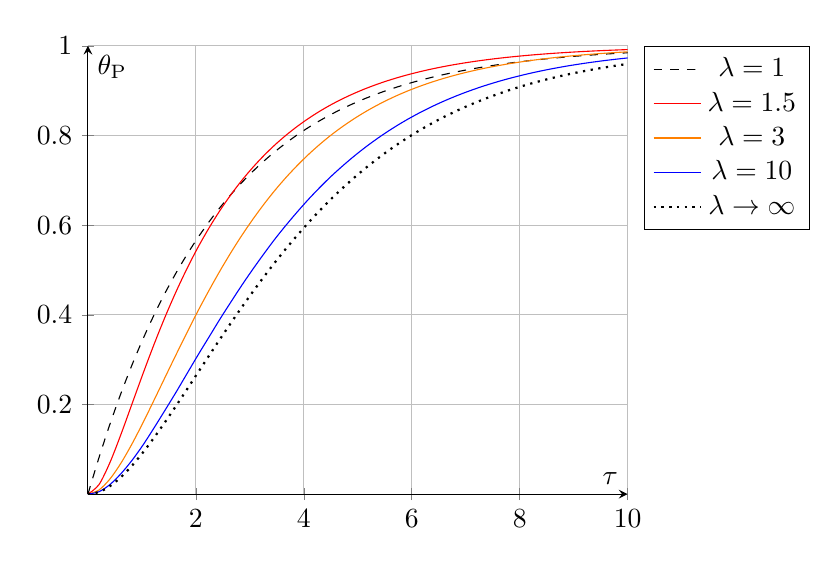
\begin{tikzpicture}
        \begin{axis}[xlabel=$\tau$, ylabel=$\thetaP$,
        domain=0:10, ymin=0, ymax=1,
        axis lines=middle,
        samples=50, smooth, grid,
        legend pos=outer north east]
            \addplot[no marks, dashed, color=black] {1-exp(-(1+1/1.5)*x/4)};
            \addlegendentry{$\lambda = 1$};
            \addplot[no marks, color=red] {1-0.5*(2.5*exp(-x/2)-0.5*exp(-2.5*x))};
            \addlegendentry{$\lambda = 1.5$};
            \addplot[no marks, color=orange] {1-0.5*(4*exp(-x/2)-2*exp(-x))};
            \addlegendentry{$\lambda = 3$};
            \addplot[no marks, color=blue] {1-0.5*(11*exp(-x/2)-9*exp(-11/18*x))};
            \addlegendentry{$\lambda = 10$};
            \addplot[no marks, dotted, thick, color=black] {1-(1+x/2)*exp(-x/2)};
            \addlegendentry{$\lambda \mathrel{\to} \infty$};
        \end{axis}
    \end{tikzpicture}
    \caption{Progress curves for varying values of $\lambda$}
    \label{fig:progress_curves}
\end{figure}

Furthermore, comparing each exact solution with its corresponding steady state solution (as depicted in Figures \ref{fig:compare_curves1}, \ref{fig:compare_curves2}, \ref{fig:compare_curves3}, \ref{fig:compare_curves4}) reveals that the steady state solution is indeed a good approximation only when $\lambda$ is sufficiently close to 1.

\begin{figure}[ht]
    \centering
    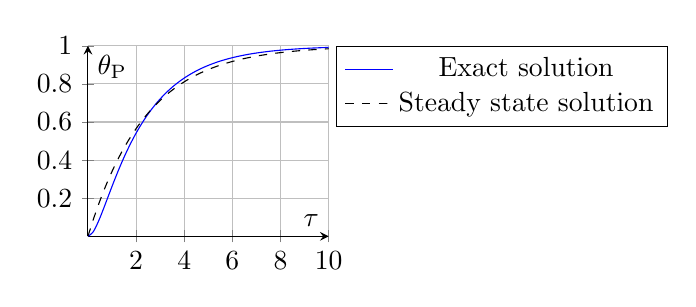
\begin{tikzpicture}
        \begin{axis}[height=0.33\textwidth,
        xlabel=$\tau$, ylabel=$\thetaP$,
        domain=0:10, ymin=0, ymax=1,
        axis lines=middle,
        samples=50, smooth, grid,
        legend pos=outer north east]
            \addplot[no marks, color=blue] {1-0.5*(2.5*exp(-x/2)-0.5*exp(-2.5*x))};
            \addlegendentry{Exact solution};
            \addplot[no marks, dashed, color=black] {1-exp(-5/12*x)};
            \addlegendentry{Steady state solution};
        \end{axis}
    \end{tikzpicture}
    \caption{Progress curves when $\lambda = 1.5$}
    \label{fig:compare_curves1}
\end{figure}

\begin{figure}[ht]
    \centering
    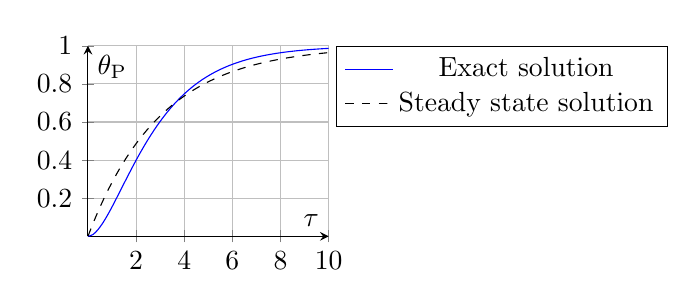
\begin{tikzpicture}
        \begin{axis}[height=0.33\textwidth,
        xlabel=$\tau$, ylabel=$\thetaP$,
        domain=0:10, ymin=0, ymax=1,
        axis lines=middle,
        samples=50, smooth, grid,
        legend pos=outer north east]
            \addplot[no marks, color=blue] {1-0.5*(4*exp(-x/2)-2*exp(-x))};
            \addlegendentry{Exact solution};
            \addplot[no marks, dashed, color=black] {1-exp(-x/3)};
            \addlegendentry{Steady state solution};
        \end{axis}
    \end{tikzpicture}
    \caption{Progress curves when $\lambda = 3$}
    \label{fig:compare_curves2}
\end{figure}

\begin{figure}[ht]
    \centering
    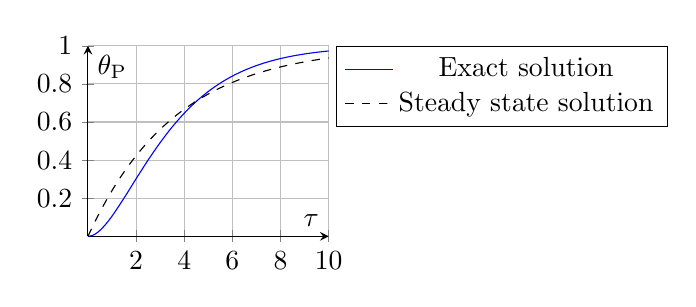
\begin{tikzpicture}
        \begin{axis}[height=0.33\textwidth,
        xlabel=$\tau$, ylabel=$\thetaP$,
        domain=0:10, ymin=0, ymax=1,
        axis lines=middle,
        samples=50, smooth, grid,
        legend pos=outer north east]
            \addplot[no marks, color=blue] {1-0.5*(11*exp(-x/2)-9*exp(-11/18*x))};
            \addlegendentry{Exact solution};
            \addplot[no marks, dashed, color=black] {1-exp(-11/40*x)};
            \addlegendentry{Steady state solution};
        \end{axis}
    \end{tikzpicture}
    \caption{Progress curves when $\lambda = 10$}
    \label{fig:compare_curves3}
\end{figure}

\begin{figure}[ht]
    \centering
    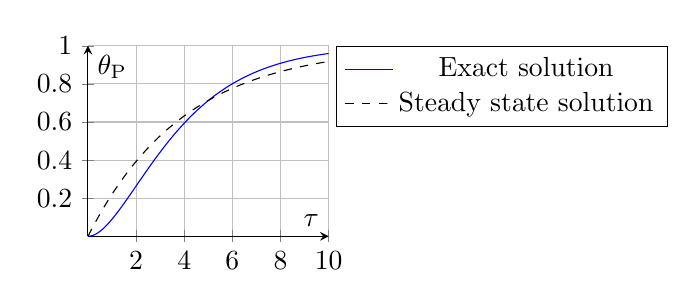
\begin{tikzpicture}
        \begin{axis}[height=0.33\textwidth,
        xlabel=$\tau$, ylabel=$\thetaP$,
        domain=0:10, ymin=0, ymax=1,
        axis lines=middle,
        samples=50, smooth, grid,
        legend pos=outer north east]
            \addplot[no marks, color=blue] {1-(1+x/2)*exp(-x/2)};
            \addlegendentry{Exact solution};
            \addplot[no marks, dashed, color=black] {1-exp(-x/4)};
            \addlegendentry{Steady state solution};
        \end{axis}
    \end{tikzpicture}
    \caption{Progress curves when $\lambda \mathrel{\to} \infty$}
    \label{fig:compare_curves4}
\end{figure}

\FloatBarrier

Now that we have some idea of how varying $\lambda$ alters the curve behavior, we can evaluate for what interval of $\lambda$ the steady state solution serves as a good approximation for the exact solution.

As seen above, it is only when $\lambda$ is sufficiently close to 1 for which the steady state approximation is a good approximation. This is easily verified by the reader by comparing \eqref{maths:eq6} with \eqref{maths:eq10} when $\lambda \to 1$: they should be equal. To better see the kinetic meanings behind the limiting scenarios, we take another perspective in analyzing $\lambda$.

\subsection{Kinetic interpretation} \label{subsection:6.2}

Recall that $\lambda$ is nothing more than a value depending on the rate constants and bulk enzyme concentration. We can rewrite it as

\[
\lambda = \frac{1}{\sqrt{1 - 4k_1^* \kcat / (k_1^* + k_1 + \kcat)^2}}
\]

Consider the limiting scenario $\lambda \to 1$. This corresponds to the case when

\[
\frac{4 k_1^* \kcat}{(k_1^* + k_{-1} + \kcat)^2} \ll 1
\]

After some rather vacuous algebraic rearrangement and substitution, we can simplify this condition to

\begin{equation} \label{maths:eq12}
\frac{k_{-1}}{\kcat} \gg \Phi
\end{equation}

where

\[
\Phi = \frac{4 \Et / K_M}{(1 + \Et / K_M)^2}
\]

A more careful mathematical analysis of \eqref{maths:eq12} reveals some special cases where this $\lambda \to 1$ limiting scenario holds:

\begin{itemize}
    \item $k_{-1} / \kcat \gg 1$ because $\Phi$ is always less than 1
    \item $\Et / K_M \ll 1$ or $\Et / K_M \gg 1$ because then $\Phi$ is close to 0
\end{itemize}

\begin{proof}
    A numerical justification using a graphing calculator like Desmos will suffice, as shown in Figure \ref{fig:func1}. The analytical proof, though, is not too confounding, so we will present it below.

    \begin{figure}[ht]
        \centering
        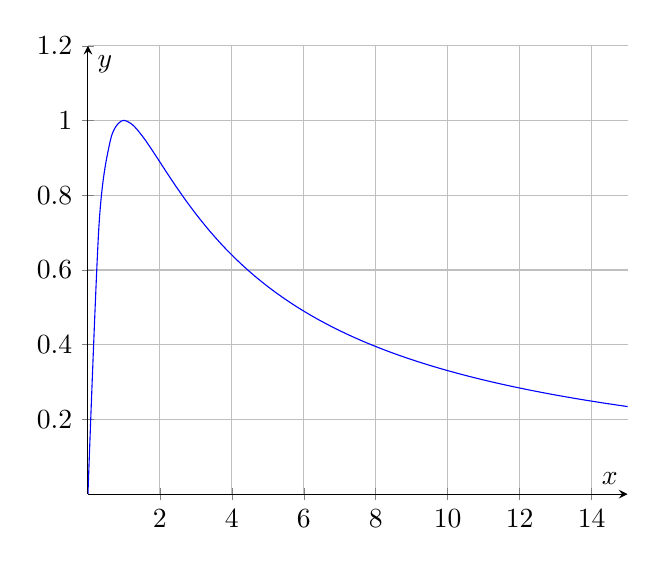
\begin{tikzpicture}
            \begin{axis}[xlabel=$x$, ylabel=$y$,
            axis lines=middle,
            domain=0:15, ymin=0, ymax=1.2,
            samples=50, grid, smooth]
                \addplot+[no marks] {4*x/(1+x)^2};
            \end{axis}
        \end{tikzpicture}
        \caption{Graph of $f(x) = 4x / (1 + x)^2$}
        \label{fig:func1}
    \end{figure}
    
    We first prove that $\Phi$ is always less than 1, justifying the first bullet point. Define function $f(x)$, of the same form as $\Phi$ for easier analysis:

    \[
    f(x) = \frac{4x}{(1 + x)^2} \text{ for } x \geq 0
    \]

    where we treat $x$ as $\Et / K_M$.

    Its derivative is 

    \[
    f'(x) = \frac{4(1 - x)}{(1 + x)^3}
    \]

    with a maximum point at $x = 1$. The graph increases from $f(0) = 0$ to maximum $f(1) = 1$, which then approaches asymptotically toward 0 from the above as $x \to \infty$.

    Thus, $f(x)$ and hence $\Phi$ is bounded above by 1, which proves bullet point 1. For sufficiently small or sufficiently large $x$, $f(x)$ approaches 0, which proves bullet point 2.
\end{proof}

The above discussion motivates the use of kinetic parameters $k_{-1} / \kcat$ and $\Et / K_M$ to describe $\lambda$, which gives

\[
\lambda = \frac{1}{\sqrt{1 - \Phi / (1 - k_{-1} / \kcat)}}
\]

This equation gives us a convenient tool for classifying the different kinetic behaviors of surface-based heterogeneous enzymatic reactions. 

\section{Using the mathematics} \label{section:7}

The shape of the experimental progress curve determines the kinetic scenario of the enzymatic reaction. If the curve is nearly monoexponential, then the steady state approximation is likely valid and we can use \eqref{maths:eq6}. The parameter $k_{\text{eff}}$ can be determined by adjusting it so that the theoretical curve matches the experimental curve. 

On the other hand, if the curve is sigmoidal, then we have to resort to the exact solution in \eqref{maths:eq9} as the steady state approximation is no longer valid. Furthermore, it may be the case that we have to use the theoretical curve associated with $\lambda \to \infty$ in \eqref{maths:eq11}. 

In all three cases (steady state, general case, full sigmoidal), fitting a theoretical curve onto the experimental curve will allow determination of the solution parameters and ultimately the rate constants governing the heterogeneous enzymatic reaction, revealing important aspects of the reaction backed with rigorous mathematical foundations.

\nocite{*}
\bibliographystyle{plain}
\bibliography{refs}

\end{document}
